\section{A Dynamic Architecture of Cognitive Agents}

\textbf{Agency: }We use the term `agent' for a physical system that is capable of action, implying thereby that not all physical systems are capable of action. Without getting into the dynamics of how this metasystem transition\cite{metasystem-francis} from physical systems to agentive systems took place, we assume that when a system does some work to maintain its dynamic organization, we consider the work done as action. This capacity implies that the system is thermodynamically open and is interpreted as far from equilibrium.\cite{prigogine2018order} The system is constantly repairing the perturbations caused by its environment through autopoiesis to maintain an organizational closure.\cite{maturana1991autopoiesis} This sense of `action' is not the same as found in Newton's third law: For every action there is an equal and opposite reaction. Reaction of Newtonian sense is not considered an action in our context.  There is a symmetry implied in this latter sense. We use the term 'action' to imply local symmetry breaking, without violating the laws of thermodynamics.  This `interactional asymmetry'  is a way of ``breaking the symmetry of its coupling with the environment so as to modulate it from within''.\cite{agency-defining} This interpretation of agent and agency is what we attribute to living organisms. This is the ground in which we identify cognitive action.  

Just as we assume there is a transition from physical systems to living systems capable of agency, we would like to further assume another transition from living agents to cognitive agents. An implication of this position is that not all living agents are cognitive agents. Describe and explain this latter transition and identify rigorous criteria for it is part of our objective.  



\subsection{A Principle of Inertia of Cognitive Phenomena}
\textbf{Action Patterns: }The unit of analysis for cognition is \textit{action patterns}, and not actions.  This requires us to shift our attention from actions \textit{per se} to \textit{change in actions}. Actions are identified or distinguished on the basis of a change in actions or simply action patterns. When we refer to the pattern, we are referring to the pattern of change, a temporal feature of action and not a static structure. 

Movements whether or not it changes the position (locomotion) of the agent, are instances of action patterns. The study of conditions required for the maintainance of these action patterns is biology, and to study the conditions that generate \textit{variations} in the action patterns are potential candidates of cognitive science.  
We assume therefore that action patterns exist in a living organism as potential candidates for participating in cognitive phenomena. For example: ciliary or flagellar movements, undulatory movement of enteron, breathing patterns of gills or lungs, heart beats etc.  These movements are localized with respect to internal as well as external environment. Localizability is a distinguishing feature of movements. 

We could then define an idealized inertial state as a model system:  \textit{A cognitive agent remains in its state of pre-existing action-patterns, until halted by either internal or external affordances.} 

Why start with this principle?  There are a couple of justifications to ground this postulate. One is the insight that \textit{differentiation of difference} is a valid condition for cognitive awareness.\cite{bateson2000steps} We could operationalize a study of motion better when we base our study on changes of speed (acceleration) than speed \textit{per se}. We do not need force to maintain an internal state of motion but to modulate it. Deviation from a pattern has more information than an invariant pattern, as an insight from information theory.  Changes and resulting differences in a living state are part of the dynamics. In such a dynamic world, changes and differences is no news, but change in the pattern of the differences could be. That is the ground for using the idealized inertial pre-existing action patterns as a canvas, upon which the cognitive phenomena can appear. 

The term `fixed-action-patterns' (FAPs) originated in ethology to describe several overt but innate (inborn) behavioral patterns.\footnote{The choice of this term becomes clear when we introduce the new term `haltable action patterns', which forms part of the proposed hypotheses.} We take the liberty to use the term to describe not only the overt behavioral action patterns, but also action patterns inside the body: heart-beat, ingesting, swallowing, peristalsis, along with the overt patterns such as walking, running, scratching, pruning, digging, swimming etc.  Considering that these are genetic, they become the \textit{action schema} available as potential \textit{concpetual shcema} for grasping the world around them.  Here, we follow the path adopted by Jean Piaget's neo-Kantian genetic epistemology.\cite{piaget-biology-knowledge}

\subsection{Actions Precede Coordination of Actions}

We make another grounded assumption that movement and action appear in living organisms earlier than their regulatory mechanisms, based on evolutionary history.  Organisms without neurons exhibit movement. Therefore, we use this as an important premise in our argument that to initiate action, centralized or distributed controlling sub-systems are not required.  

Dynamism is rooted in the deeper layers of ontology in physical and living world.  So, we postulate a counter-intuitive principle: actions are natural, and they don't need a triggering message or mechanism to act, but they are required for \textit{halting} them. This is analogous to the dynamical first principles of physics; maintaining inertia doesn't need force but it is required to modify its course.  

We see a pattern in the evolutionary history.  Organisms that arrived early in evolutionary history show more uninterrupted action patterns than those that arrived late. The greater coordination of actions we see in the recent organisms exhibits a greater variety of interrupted action patterns. This indicates an insightful connection between coordinated action and haltability of action.\footnote{We prefer the term `coordination' instead of `control', since our position has greater affinities to distributed and decentralized explanatory models than a centralized one.} Single-celled organisms are more dynamic but exhibit fewer action patterns. Multicellular organization introduces constraints in uninterrupted movement but enables new \textit{syntax} in the possible action patterns by introducing \textit{gaps}.  Dynamic synchronous actions become more difficult than alternating or undulating actions in a `society' of multiple cells.  The shapes organisms take directly reflect on the action patterns. We will demonstrate how these haltable patterns play a role in cognition.\footnote{It is tempting to discuss the role of action patterns in the shapes organisms take and the dialectics of movement and form, but we will restrain ourselves from this temptation and focus on discussing the cognitive role the action patterns play.}   

\subsection{Antagonistic Architecture could Generate Fixed and Haltable Action Patterns}
We have sufficient ground to assume multiple action zones are acting on and affecting each other in an agent's body based on our understanding of comparative animal anatomy.


Antagonism as an explanatory theme in biology is widely recognized. The role of agonistic and antagonistic muscles in motor coordination is well established. Each action zone may have multiple sets of agonist and antagonist \textit{actors}.  A contraction leading to a pull of agonist alternated by an antagonist's pull may generate a simple open-close pattern, one cycle: one fixed action pattern (FAP). It may be noted that muscles can only pull when contracted, and no push action is possible. A counter-acting muscle, an antagonist, pulls it for the following action cycle. 

This can be modeled as a Petri net, a bipartite graphical representation used widely for modeling processes as changing states are affected by transitions. The two kinds of nodes in the graph are places and transitions. A transition has a prior state represented as an input place value (token) and a post-state as a resulting place value. Thus, a process or an event is represented as a transition of places from prior to post state. The prior state is interpreted as a necessary condition for the transition to happen. The result can be a pre-condition for one or more transitions leading to a network or a chain of transitions.

For example, a sense organ as a transducer can be represented as a transition of an analog physical perturbation from the environment (an input) into an action potential within the agent. This transduction is the basic source of input tokens to the agent, forming sensations.
\begin{figure}[ht] 
%\renewcommand{\thefigure}{2}
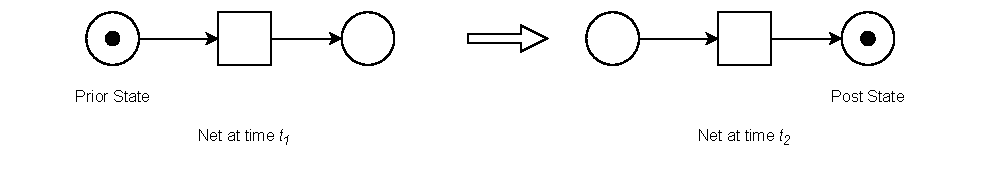
\includegraphics[width=\textwidth]{graphics/PN_Transduction.pdf}
\caption{\textbf{Transduction:
}The transducer is represented as a square node, which will fire when a condition of at least one token as input place value is satisfied, giving rise to the resulting place value.
Places are represented as circles with or without tokens (the values).}
\label{transduction} 
\end{figure}


A coordinated Pair (CP) generating FAPs
A coordinated Pair (CP) generating HAPs
How FAPs become HAPs



However, a pull action from the complement muscle between the cycle can generate a halting action in between.  Thus two actors can regulate each other's action without involving any other controlling agent or actor. If the pulling forces are equal and opposite, we may expect a jam, but variations in the pull may generate a resulting vector. A fine-grain halting may lead to greater coordination.  This is one model of implementing a simple haltable-action-pattern (HAP). \footnote{Citations to such explanatory models in kinesiology or mechanical engineering or robotics will be helpful.} 

There are two senses in which multiplicity plays an important role. One sense is similar FAPs at multiple locations (zones) of the organisms' body. The second is in the sense of variations among the zones based on action patterns.  For example, a biting action of the mouth differs from a waving action of the tail zone or a walking zone of limbs, while multiple walking zones exhibit similar patterns.  We use this sufficiently grounded assumption based on comparative anatomy of organisms to postulate the following \textit{dynamic principle of antagonism.}

Haltability, coordination of actions, emerges due to dynamic antagonism among the zones.  

\subsection{Body as a differentiated torus}
Most multi-cellular organisms during the development indicate that the underlying form is that of a torus. Specialized morphogenesis, leading to differentiation, the final shape appears differently. 

The broad body plan of a cognitive agent is tubular and topologically a torus. [Refer to wireframe diagram of C.Elegans]. A tubular architecture offers an inner as well as outer layer and the middle layer in between. The 3 components of concern for a cognitive architecture are (1) the sensory receptors organised as \textit{sensory boards (SB)}, (2) the motor action zones organised as \textit{motor boards (MB)} and (3) the connectors in between sensory and motor boards organised as a \textit{network}. Thus the body of a cognitive agent is modelled as a sensation modulating network (SMN). The nodes of the network include sensory and motor boards, while the edges include the connections of the network. Biologically, sensory boards are realised by sensory receptors, motor boards by the muscular and skeletal system and the edges of the network (connections) by the nervous system. It is important to keep in mind the contrasting point of the architecture with the received view that confines network only to the nervous systems, where the body of the neuron, the soma, forms the node, and the axons and dendrites form the connections.



The core proposal is to show that there exists a world within the body and a clear criterion of demarcation between the internal and external worlds. By doing this, we demonstrate that behavior is not restricted just between the body and the external world, but included action performed within the internal environment of the body. We demonstrate this possibility by modeling the body of a cognitive agent as \textit{a network situated in an environment} which includes other agents and physical systems. This is in contrast to the widely received view of a centralized computational brain controlling a sensory-motor body, which, in turn, interacts with the world out there.

The grounding of representations that we are attempting is achieved by remodelling the biological architecture (anatomy and physiology) of the body itself, in order to make internal environment possible.

\subsection{Biological Architecture for Cognition: Tubular, Polarised, Nested, Serial and Bilaterally Symmetrical Body Plan}

% \footnote{Contrast with brain-body-world schema} 
The broad body plan of the SMN is tubular and topologically a torus. [Refer to wireframe diagram of C.Elegans]. A tubular architecture offers an inner as well as outer layer and the middle layer in between. The 3 components of concern for a cognitive architecture are (1) the sensory receptors organised as \textit{sensory boards (SB)}, (2) the motor action zones organised as \textit{motor boards (MB)} and (3) the connectors in between sensory and motor boards organised as a \textit{network}. Thus the body of a cognitive agent is modelled as a sensation modulating network (SMN). The nodes of the network include sensory and motor boards, while the edges include the connections of the network. Biologically, sensory boards are realised by sensory receptors, motor boards by the muscular and skeletal system and the edges of the network (connections) by the nervous system. It is important to keep in mind the contrasting point of the architecture with the received view that confines network only to the nervous systems, where the body of the neuron, the soma, forms the node, and the axons and dendrites form the connections.

Sensory receptors are located in a distributed way across the body in the outer, inner and middle layers. The distribution of these nodes \textit{on} and \textit{in} the body is not uniform. Polarization exists, in the sense that some nodes are arranged densely on one-side of the tube. The sensory receptors are differentiated into specialised modalities transducing thermal, tactile, auditory, visual, olfactory, gustatory and location signals. The polarised and bilaterally symmetrical arrangement of these sensory receptors plays a significant role in constructing the picture of the internal and external world. The receptors organised as sensory boards are \textit{mounted} on the motor and mechanical boards (muscular and skeletal system). For example, a pair of eyes are located towards one pole of the body and absent at other places. Each eye has multiple photo-receptors and motor modulators, together constituting the nodes of the network. Similarly we see such concentrations of sensory receptors for other modalities. Although tactile receptors are located in a distributed way, their density varies from place to place on and in the body. This unequal distribution in location and density of sensory receptors plays an important role in differentiation and solving the problem of location. [Make a picture of praying mantis]. One more contrasting point of this model may be noted, that we consider the motor boards as sensory receptors of location, and not merely as actuators. As far as cognition is concerned, actuation is essentially for supporting sensation of every modality, committing to the theory of action based perception.

On this body plan, there are also multiple action zones. It is important to note that action zones are also oriented towards the inner layers of the tubular body plan of the agent. There are more action zones at the anterior side, particularly at the inner surface of the tube, making the body polarized. Animal anatomy describes this plan often in the name of cephalization, seen in almost all bilaterally symmetric beings. The significance of a polarized body plan and the existence of action zones at the inner surface becomes clear as we discuss the modulation mechanics below.

The schematic shown in figure~\ref{smn} shows a typical cognitive agent's polarized and bilaterally symmetric body plan, based on the model described here. Motor boards are present all over the body attached to the skeletal system that facilitates movement, while the sensory boards are mounted on moving structures at several action zones of the body. The term action zone is used in this article to refer to a complex of flexing areas, which are often located at an identifiable place in the body. For example, orbit of an eye, lip- movement, flexing the digits or toes, holding an object etc. [Based on the figure: We represented an assembly of motor boards as rectangular action zones at the interface of the body and the internal and external environment in the figure.]

Apart from the polarised distribution of sensory organs, it is important to note that the motor organs, which are also sense organs, are located in a \textit{nested} manner across the body.
A large set of highly specialized motor receptors (location sensors), are present across the body organized in a bilaterally symmetrical and hierarchical (nested) manner, which biologists call as skeletal or voluntary muscles. [Add a citation that supports the tree for skeletal and muscle anatomy.] In our model, insofar as cognition is concerned, skeletal muscles are sense organs, and their movement directly supports perception.  Biologically, muscles are considered as organs of movement and locomotion. In conventional cognitive science, their role is considered auxiliary. In our model, movement and locomotion are primarily cognitive functions. Apart from providing location data as a sensory subsystem, their \textit{characteristic} movement provides conceptual schemes employed in cognition. As this is a central and contrasting feature of the model, more elaboration on the characteristics of the movement are presented below.

The motor receptors of the network are unique, because they are mounted/embedded in a bundle of muscle fibres organised as \textit{boards}. This specialized plan is essential for playing the role of \textit{inferring} the location. The data from location sensors is created through movement. That is to say, the position is resolved only by change-in-position (displacement). But, location cannot be determined without data from the other sensory streams. We interpret location, like consciousness, as a dispositional concept. Location is always of some thing or the other, some sensation or the other, of some phenomena or the other. Employing a Kantian aphorism, we may say: location without sensory data is empty, and sensory data without location is blind. Moreover, it is not only that location cannot be calculated without movement, the construction of an image of the world through other senses is impossible without spatio-temporal data. Action is essential for resolving both space and time. What makes an action possible, is a foundation question, but it is beyond the focus of this paper.

\emph{Elaborate on synchronicity and serial aspect of the actions to resolve time.}

The source of temporal data is the serial action pattern.The body plan is not only polarised and nested, but also serial in nature. We also assume availability of repeatable actions, beats within the body, providing a temporal canvas/ stage. The availability of the temporal stage/ canvas is granted by the existence of metabolic cycles, biological clocks is well established [cite] in terms of diurnal and biurnal rhythms.\footnote{need to elaborate with right vocabulary and cite relevant sources}.


Antagonistic action is a key character of the body plan, which plays an important role in the current model. 

The body is not a complete network.\footnote{In graph theory, a complete network is defined as a graph where each node is connected to every other node.} Some SMNs are connected to only certain others. The model uses the principle: ``Fire together. Wire together'' (FTWT) \cite{hebb1949organisation}\emph{Principle: Fire Together Wire Together}. The SMNs that are recurrently active at the same time are likely to get connected over a period of time. Thus the connection `board' is plastic, not static. The connection patterns are created, reinforced and modified based on the dynamics of the body (action patterns) in its ontogeny (developmental history). The implication of the FTWT principle is that the actions determine the connections, and not the other way around. However, much of the differential connections may have been already determined by phylogenetic and prenatal action history. Though it appears as though the agent starts with an undifferentiated state, the phylogenetic and prenatal action history bestows, practically, a body with `innate' action schemas at birth.\emph{Affinity with Nativism} In a model where actions are located at the interface between the body and the environment, the actions within the body (including the prenatal stage) are often ignored (e.g. suckling, swallowing action-patterns etc.). In our model, the most stable and determining action schemas are already in place by the time the agent is exposed to the external environment after birth.

The array of receptors as a board are connected by an incoming bundle of sensory neurons to the DFN as shown in the figure.


We shall discuss the origin of differential connections and various possibilities of their implementation in the section~\ref{mbr}.

In the schematic shown in figure~\ref{smn} the connections within the IN are not drawn to avoid clutter. The arrows between action zones (Z-A to Z-H) represent modulation of the zones, and not the connections. 

\begin{figure}[ht] 
%\renewcommand{\thefigure}{2}
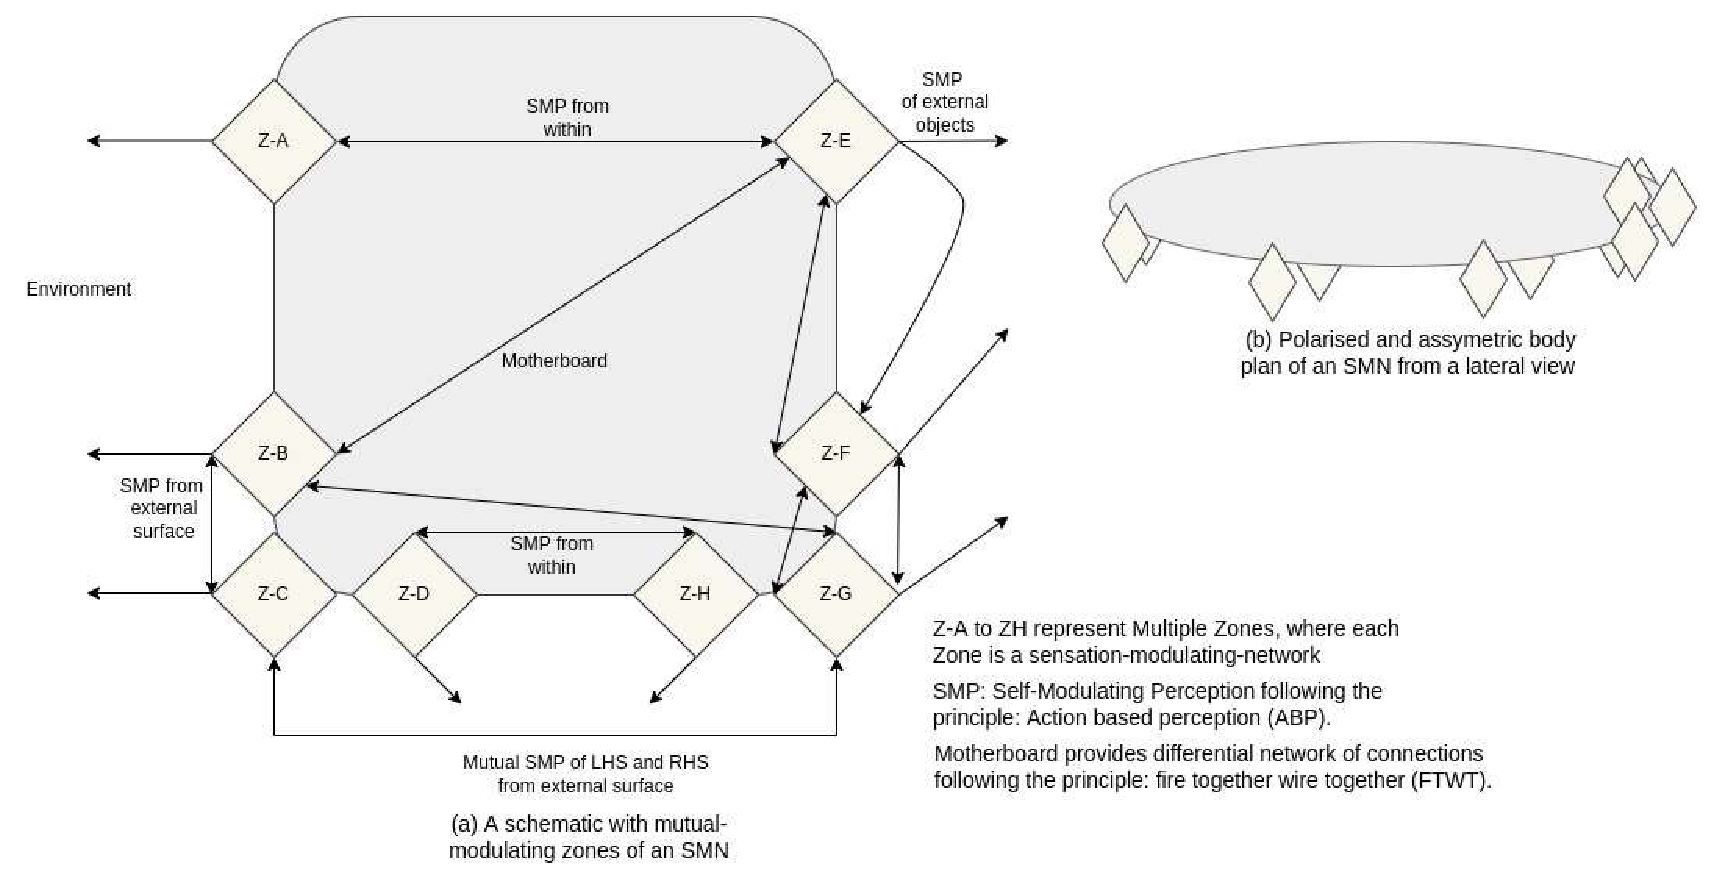
\includegraphics[width=\textwidth]{self-modulating-perception.pdf}
\caption{\color{Gray} \textbf{A schematic representing a cognitive agent as a network of multiple self-modulatable zones.}}
\label{smn} % \label works only AFTER \caption within figure environment
\end{figure}

The outgoing arrows from the zones represent the sensory modulation from an external world invoking action based perception (ABP) \cite{noe_action_2004}\emph{Principle: Action-based Perception}. According to this principle, the perception is not a passive sensing of the world out there, but an active process.

The same principle is employed when an action zone modulates another action zone within the body. This implies that ABP is used for perceiving both the worlds (internal and external). The double headed arrows in the figure represent mutually modulating zones. Between Z-B and Z-C, the double-headed arrow represents mutual modulation from the outer surface. For example, consider a fidgeting action between fingers touching side-ways, the hand touching the chin in the typical thinking posture, scratching an itch on the same side of the body etc. The double-headed arrow between Z-C and Z-G represents another mutual modulation from an outer surface (e.g. clapping with hands), LHS and RHS mutually modulating.
In a well-connected body, the implementation of a single-headed arrow between two zones (like Z-E and Z-F) appears very rare. However, to understand such a possibility, we can consider touching a numb leg, where due to temporary lack of internal feedback, mutual modulation is transiently unavailable.

The double-headed arrow between Z-D and Z-H could represent mutual modulation between the action zones from within the body. For example, swallowing zone and speech zone. In the case of swallowing, with or without food, the upper and lower surfaces of the buccal cavity, pharyngeal zones mutually touch and modulate each other.

\emph{Principle: Body-plan as torus.} But it is very important to realise that this internal and external distinction would vanish when we bring to our attention the topological architecture of the body, which is a torus. Therefore, the apparently internal surface of the body is topologically external. 

Mutual modulation of action within the body is an important and contrasting feature of the model, which is largely ignored in the current discussions in cognitive science.\label{contrast-internal-ABP}\emph{Principle: Self-modulation.} This mutual modulation, within the body, is a core cognitive mechanism in the current model, which appears very early on during the prenatal stage itself. Therefore, we locate the roots of cognition within mutual modulation within the body (internal environment). 

Often, self modulating actions, such as thinking, are considered as recent evolutionary features, whereas in our model, the very root of cognition is due to such internal mutual modulation, though it is counter-intuitive. The world within the body is missed in the current accounts. Since this is a contrasting feature, more elaboration on this follows in the model.


We described the body as a network of sensory and motor boards. We provided an indication of how the body acts on itself and with other things in the world.  We will now turn to describe the details of sensory modulation. 

\begin{figure}[ht] 
%\renewcommand{\thefigure}{2}
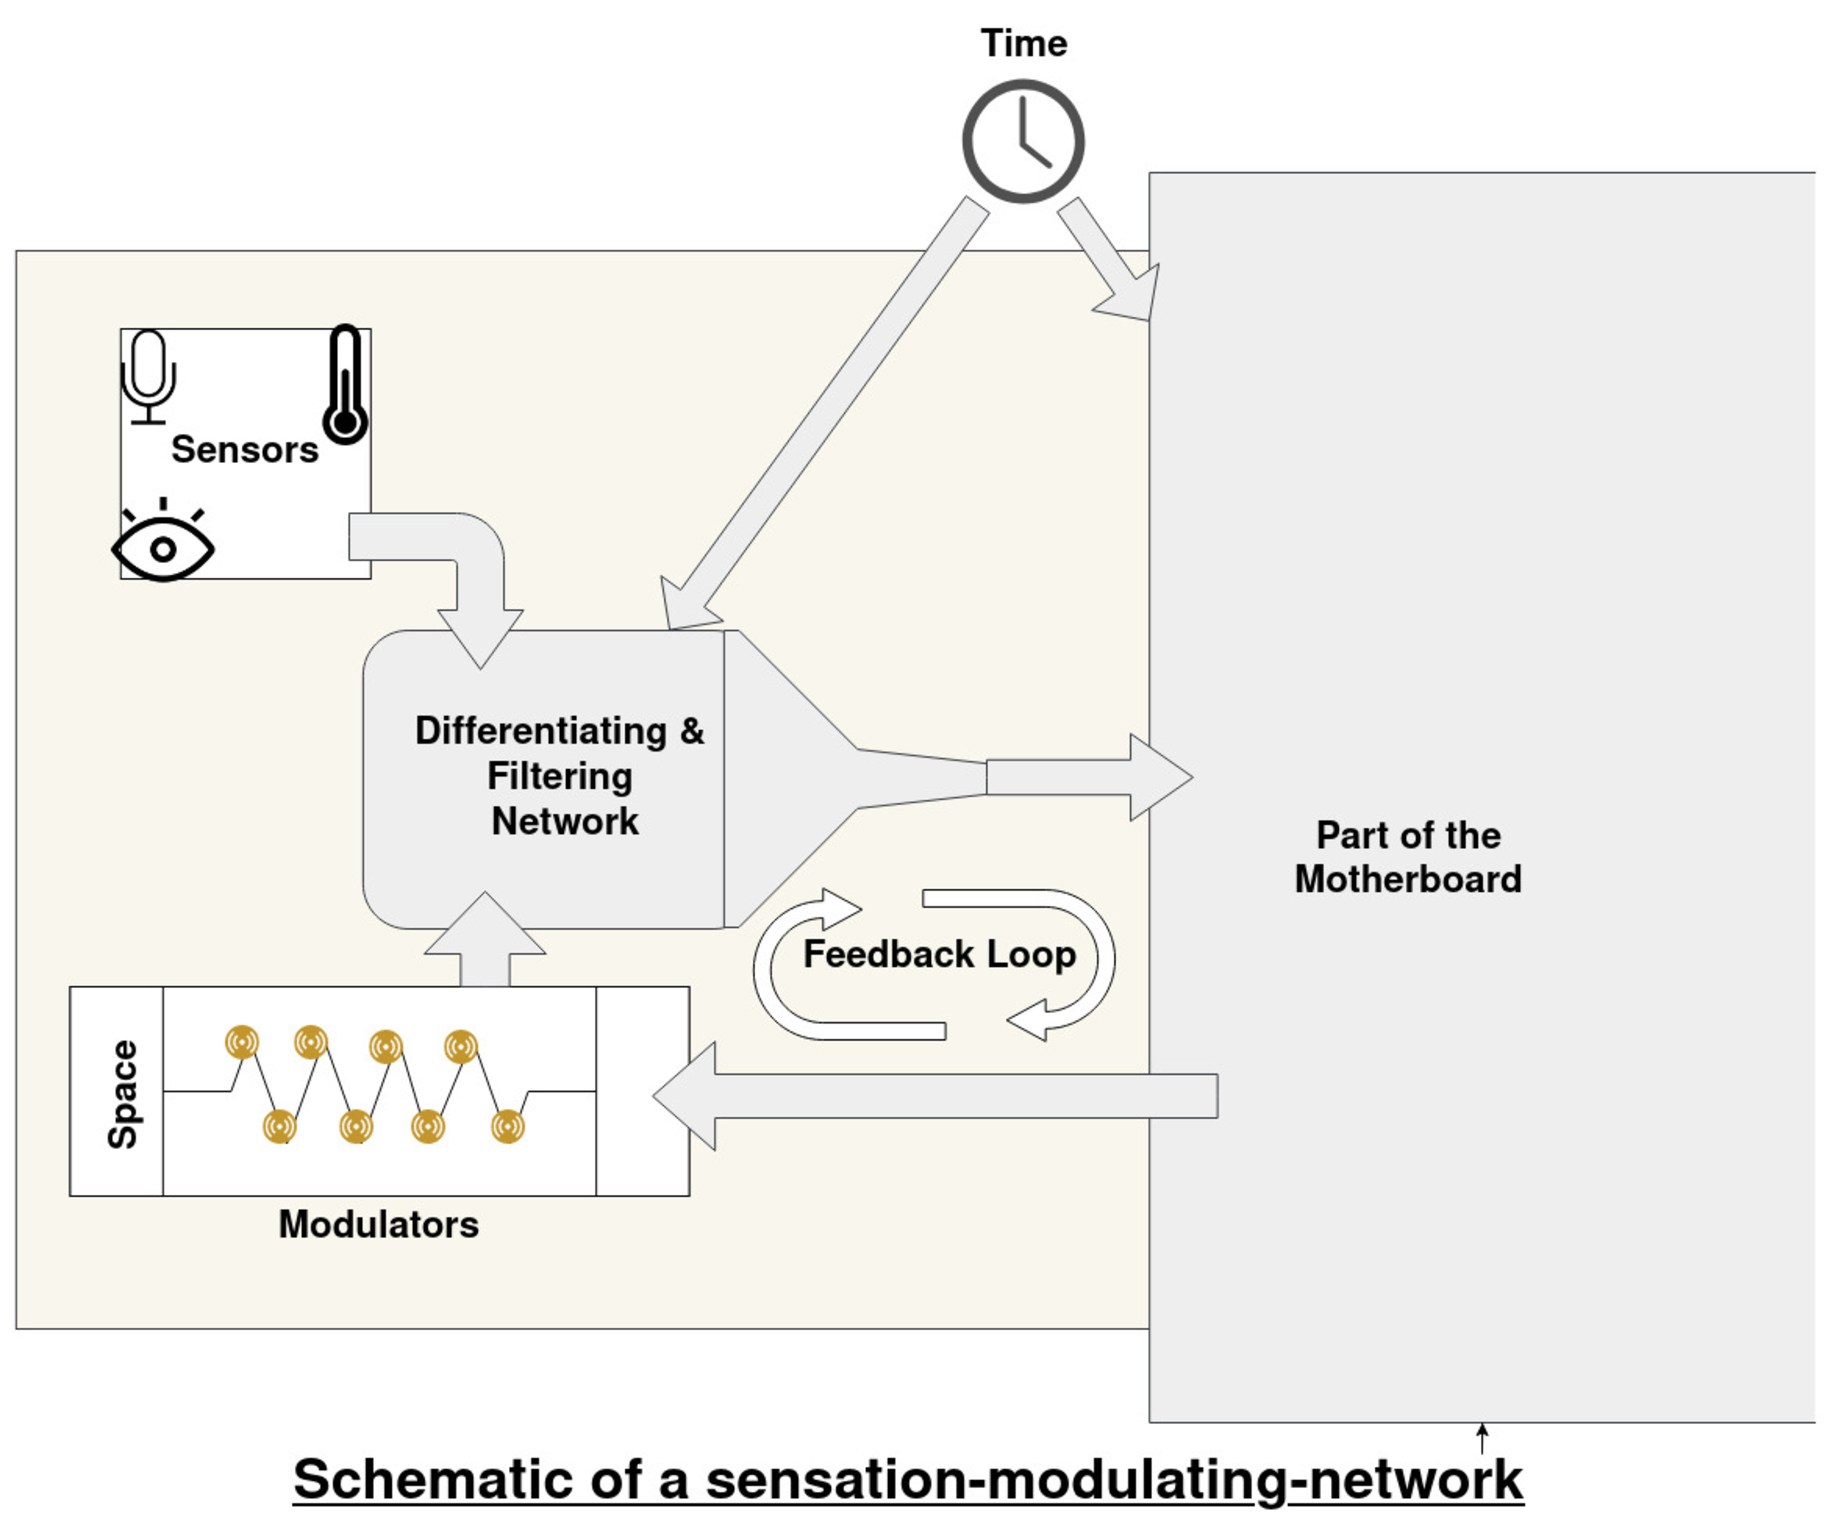
\includegraphics[width=\textwidth]{structure-of-Zone.pdf}
\caption{\color{Gray} \textbf{A schematic of a perception modulating action zone.}}
\label{zone} % \label works only AFTER \caption within figure environment
\end{figure}

\subsection{A Network of Sensation modulating networks}

\subsubsection{}

The structure of a cognitive agent's body is modeled as a nested network of Sensation Modulating Networks $\{n(SMN)\}$. And the dynamics of cognition is modeled as differentiation of Differences $\{\delta(D)\}$ in a  multi-modal sensory stream.

It is important to underline, as a point of contrast, that the Central Nervous System (CNS) is not interpreted as \textit{the} network in our model, but a part of it. The entire cognitive agent's body is a network. CNS provides only the differential connections between different DFNs and among the nodes (sensory and motor receptors). Therefore the popular schema of brain-body-world is reduced to body-world. Since the body is a network of SMN, this schema can be represented as 
\begin{equation}
[\{n(SMN)\}\rightleftharpoons \{W_I\}] \rightleftharpoons \{W_E\},
\end{equation}

where $W_I$ is the internal world and $W_E$ is the external world.  $W_I$ can be substituted with another $\{n(SMN)\}$, since it is nothing but another $W_I$ in effect. 


Thus the above representation can be re-written as 
\begin{equation}
[\{n(SMN)\}_i\rightleftharpoons \{n(SMN)\}_j]\rightleftharpoons \{W_E\}.
\end{equation}
What constitutes the internal world will become clear once we make the principle of mutual modulation clear below.


This schema can be contrasted with the brain-body-world schema, which can be represented as 

\begin{equation}
\{CNS\}\rightleftharpoons\{B\}\rightleftharpoons\{W_E\}
\end{equation}

where the CNS is the central nervous system, B is the rest of body and $W_E$ is the external world.

Consider the functional network as a $\Delta$ network of a set of sensory boards $\{S_i\}$ and motor boards $\{M_j\}$. We represent this network as \begin{equation}\label{delta_notation}\Delta^{\{S_i\}}_{\{M_j\}}, or simply, as  \Delta^{\{i\}}_{\{j\}},\end{equation} where the subscripts always refer to motor boards, and superscripts to the sensory boards. For example, if $S_1$, $S_2$, $S_4$ and $M_1$, $M_5$, constitute a transient network at any given time $t_1$, this state of the SMN can be represented as 
\begin{equation}\label{delta_eg}SMN(t_1) = \Delta^{1,2,4}_{1,5}\end{equation} This $\Delta$ network is an ephemeral functional state corresponding to a particular action performed by the cognitive agent at $t_1$. Thus differentiation of Differences is realised in $\Delta$ networks, where the motor boards differentiate on the Differences streaming from the multi-modal sensory boards. This is how we resolve every action as a functional network of sensory motor subsystems.

Differences are given and taken from the environment directly, while differentiation is an active function of the agent. This active function can resolve modalities and selectively attend to a difference in the stream.

SMNs are functional states of the cognitive agent. This identifiable functional state does differentiation and filtering. Since each SMN is a network, the body is a network of networks. We may represent the active cognitive agent as $\{n(SMN)\}$. The first order network of SMN is a functional sub-graph. By functional subgraph, we mean, it is not distinguished based on structure, but by ephemeral or transient connections. SMN is hence localizable, but ephemerally.

An analogy with modern communication infrastructure helps here. When a group of people are present in a global online meeting, the people are connected through their devices. The people and their devices are localized in space, but available to other locations at about the same time. A bunch of ISPs (Internet Service Providers) enable these connections through networking boards called routers. Though the networking routers of each of the ISPs are distributed geographically, the location of the networking router is not relevant, as long as the router is accessible to the devices. Some of them may be connected through mobile networking access points, while others are connected through copper wire, and yet some others through optical fibre. How they are connected is not relevant, as long as they are connected somehow.

In a cognitive agent's body, the location of sense organs may be distributed anywhere in the body. The stream of signals coming from them at a given time is part of the \textit{cognitive engagement} only when the sense organs are modulated. Though the existence of neurons (wiring) determines connections, the actual connection gets established when the wires actually get fired at the right time. What visual or auditory stream is available at a given time is determined by what actions are carried out at the time. The sight and sound stream, e.g., should be tuned to a situated action.
Considering the actions such as talking, walking, turning etc. as determiners of active connections at a given time, we consider an SMN as a dynamically actualized region of the possible networks the body plan offers. Just as the subscribers of an online meeting are registered by seeking to be part of the meeting, in a cognitive engagement only a set of the stream of sensations are considered a part of it, while the rest are ignored. We shall elaborate this mechanism below.

Let us be warned that the analogy with an online meeting is employed only to bring home the point that the SMN is a dynamic network actualized among the possible configurations of the body plan. Just as the connections established for a specific online meeting is one of the several possibilities the Internet offers, the SMN is a dynamically actualized network formed transiently among the various possibilities the network provides. The network is not a localized structure, though the nodes of the network (motor and sensory boards) are. As we proceed further, we shall take more examples to gain clarifications on the structure and dynamics of SMN, which may differ from the online meeting analogy used here.

When an SMN is described in terms of its function, we can expand the acronym as sensation modulating network. In terms of the structure a cognitive agent's body can be described as sensory motor network. The expansion of acronyms can therefore be contextual. For example, the functional network is of $\Delta$s, and the structural network is of the sensory motor boards.

Each sensory board is an array of localised sensory receptors (transducers), which connect through a bundle of connectors (a bus) to a differentiating and filtering network (DFN). Each motor board is an array of location-receptors mounted on a bundle of actuators (muscle-fibers). The motor board connects through a bundle of connectors to the DFN on the one hand, and receives connections from the integrating network (IN) on the other. The DFN and IN are distinguishable only on the basis of their function and the nature of connections, and need not be localized in any specific area of the central nervous system (CNS).

The motor board can be considered as a mediating board between a DFN and IN. In other words, the motor board is sandwiched between the DFN and IN, creating dynamic and transient loops. Speaking of the network in graph-theoretic terms, we can say that, the nodes of an SMN are arrays of receptors and actuators, and the edges are dynamically distributed bundles of connections manifesting the aforementioned loop.
Though the network appears bilaterally symmetrical, the SMN extends both sides. The connections can be distinguished into those that come from the receptors (sensory as well as location sensors in motor boards) to the DFN, and those that come from the IN to the actuators.




\subsection{Sensation Modulating Network}
Let us recall that the units of modulation, namely SMN, may be located in a distributed manner, and therefore the boundaries of SMN are identified and defined only on the basis of how the components of a unit are connected to each other, and not on the basis of their location. Therefore, to be considered part of an SMN, the components can be anywhere in the body. The boundaries of zones are defined only functionally, not anatomically. It is identifiable only as a dynamic sub-graph of a network, thus making the network ephemeral. The figure~\ref{zone} describes the sensation modulating network.

The difference between mounting and being connected may be clarified through a thought experiment. Sense organs have to be mounted on a moving part of a body, or a moving body. This is necessary for sensory modulation. In the absence of sensory modulation, the information stream passing through the sense organs remains unprocessed.

The sensory (transducers) boards are specialised for a specific modality, such as light (visual), sound (auditory), smell (olfactory), taste (gustatory), touch (tactile) and location (spatio-temporal). The motor boards are modulators (actuators) and are transducers for location data. The clock at the top indicates the availability of time to the system. Thus time, location and other sensory modalities are available to the differentiating and filtering network (DFN). DFN connects to other SMNs through the IN. {The connection between locating, addressing, attention, naming, retrieval, re-moving, memory, recollection, etc. needs to be elaborated at an appropriate place.}

The stream of sensations/signals, which is a result of transduction, enters this network undifferentiated. What is transduced is determined by the limits of the transducers, which developed evolutionarily. There are biochemical activities that keep the transducers charged and refreshed. Though it is passive from a cognitive point of view, it is not passive from a biological point of view. 

For example, the transducers (rods and cones) in the retina have to be in a polarised state prior to light falling on them. The light perturbs and depolarizes them, which generates a stream of signals. The refreshing process of repolarization is a process of compensation/repairing/restoration. During this period of restoration, the transducers are incapable of generating any signal, even if environmental inputs are present. This layer of activity is metabolic and does expend energy for its maintenance to keep the zone active. The mechanism at this layer generates \textit{differences}, but no differentiation takes place. 

An implication of this for cognition in our model is that it is not available for conscious cognition, though the adaptive biological aspects of life are available. The adapted environment where the organisms could live/sustain depends on the availability of the refreshing metabolic process. When such a process is not available, the sensory differences required for cognition are also not available. Though the organism spends energy for the refreshing process, this is affordable to the organism. If the process of sensation itself is more expensive than the basic survival mechanisms, the variations would not have evolved through natural selection. This means that another layer of metabolic activity exists that makes the sensory mechanism available. The frequency of refreshing cycles at this physiological layer must be higher than the refreshing cycles of the sensory layer. Unless the deeper layers generate a sufficient surplus, the upper layers may not remain in an active state. An implication of this layered ontology is that the conscious cognition depends on the surplus made available by the core metabolic layers.

The range of sensations that are possible for an organism depends on the refresh/repair mechanisms available to it. For example, the spectrum of sound or light, or the extent of touch that the organism can differentiate, must fall within the economic zone of refresh/repair mechanisms. When the organism is exposed to extreme ends of the spectrum, there exists a potential danger for survival, since the repair mechanisms don't exist. \footnote{Apart from survival, the aspect of aging/functional changes – both positive and negative – can be explicated.}

The above elaboration portrays the dependency relation between the physiological and sensory layers. We now turn to the next point of dependency relation between the sensory/transducer layer and the motor/actuator layer. Thus we move from differences to differentiation. 

When actuators move, there is a corresponding change in the input stream. The action \textit{interrupts} the stream. Whatever sensory stream that enters at the time of action becomes phenomena. The entire stream does not constitute percept, but only that which is acted upon. Thus this process is active, not passive. One effect of this action is filtering. \emph{The world may have a rich structure but it is not accessible to the agent until acted upon through cognitive exploration. Move it to another appropriate place in the article.}

Apart from filtering, actions can also resolve the structure in the phenomena because the actions may not be monotonous, they may have a pattern. The changes in pattern can resolve details available in the phenomena. The change in pattern can be in terms of temporal characteristics like pause, frequency or speed. Grasping the structure in the phenomena corresponds directly to the action patterns. The poorer the action patterns, the poorer the structure of the phenomena will be. Though the structure of the phenomena is constructed, it cannot be generated without a corresponding structure in the world. 

In a cognitive model, not using ABP, richer action patterns in an empty external world should not produce a phenomenon. However, in our model, actions always generate phenomena, because every action perturbs the internal world. Thus differentiation due to action works only when the objects \textit{out/in} there can be differentiated. Absent variations cannot be generated purely out of richer action patterns.  But, without actions there are no phenomena. We shall see later (a) how we may explain what we perceive in a dream (b) how the criteria between \textit{out} there and \textit{in} there can be differentiated. 

Another vital role of the actuators is to differentiate the incoming stream of signals into different modalities. The changes in the sensory stream at the time of action, can be obtained by differentially and recurrently modulating the sensory stream.
For example, moving the head sideways, or moving the eye ball in different directions, moving close to/ away from the source of sound, closing eyes/ears etc., impacts changes in the sensory stream. The change in the visual stream, at the time when the head or the body moves, is differentiated from the change in other modalities. The apparent independent changes in the stream of any sensory modality while moving are differentiated just on the basis of the corresponding rate of change. Holding some aspect constant, while changing another aspect, is modulation. An analogy of this model with the nature of experimentation will be discussed further in the next section.

Thus, modulation does two more things apart from filtering (attention). One, it helps in differentiating the signals into different modalities. Two, it helps in calculating the rate at which each of the modalities are changing in a given stream. All the three operations, filtering, separating modalities, and correlating with the rate of change, are part of an active cognitive processing, which can be called \textit{differentiation of the differences}\emph{Cognition is differentiating the differences}.

The active processing done in cognition happens in the DFN. The filtering process economises the amount of processing required for cognition. The result of this is a richer set of a stream of differentiated data about the environment, which passes onto the IN.

The DFN does the filtering and differentiation due to the motor boards available all over the body, modulating the sensations. We are only ascribing a descriptive role to the DFN, without explicating the detailed mechanism describing exactly how it happens. However, the speculation is grounded, because we know from electronics that networks are capable of computation, depending on the differential nature of logical connections.  We propose that the data is constructed by the DFN by involving the mediating and modulating motor boards as nodes of the network. What happens in DFN is active while what happens in IN is passive. Passive doesn't mean insignificant, but no further processing is required. What happens from the IN is a composite self, a very significant emergent outcome. 

Often the current models recognise only touch, vision, gustatory, auditory, olfactory and proprioceptic sensations. Thus, the modulatory part of the body, such as muscles, provide only proprioception. However in our model, we consider actuators as fundamental sense organs providing spatio-temporal information not only from within the body, but also locating the body in the space-time with respect to the rest of the external environment by providing space and time information. We shall elaborate exactly how this demarcation of internal and external environments happens in the next section.

We make an assumption that the location information (position) is sensed not by direct observation, but through displacement (a measure of change of position). Given this assumption, if there are no action generating actuators, and if there exists no differentiable sensory stream the position sensors on them generate no useful information.

Why computing location is such an important process of cognition? Our argument is based on the assumption that atemporal pattern, such as a picture, is a constellation.  In a constellation the spatial relations between various elements are held constant. A recognition of a pattern depends on recognizing the constellation of relations, which are invariant.  E.g., face recognition. The various pieces of the face and their positions can be arranged logically in various ways. Unless the pieces are placed relative each other in a correct way, we cannot coherently regenerate the face. Keeping the pieces of the face constant, if we change the spacial relations between them, we can generate different faces. This geometrical transformation applies not only in understanding faces, but also the evolution of variations of forms in the living world.\cite{thompson1942growth} It is through a calculus of dynamic transformations we grasp geometrical patterns in the world.

As stated already, there are multiple SMNs in the cognitive agent's body, which is modeled as a network of SMNs. All the SMNs are connected through the IN, which provides an integrating and differentiating experience depending on the nature of connections. The analysis of experience happens at the SMNs, while the interconnections in IN provide the synthesis. As mentioned earlier what happens in IN is passive, while what happens in DFN is active. Maintenance of polarity of wiring of the network does need a lot of activity, but this activity happens at a core metabolic layer of the body. The networks are power hungry, since each firing of signal discharges the wires. It is assumed in this model that maintaining the potential by repolarizing or refreshing them happens by the metabolic activities of the biological layer. Cognitive layer depends on the biological layer.  We shall see in the later section that this separation of cognitive actions from biological actions happens through affordable disengagement.

{\emph{ Write Summary of the model section}

